\documentclass{standalone}
\usepackage{tikz}
\usepackage{ctex,siunitx}
\setCJKmainfont{Noto Serif CJK SC}
\usepackage{tkz-euclide}
\usepackage{amsmath}
\usetikzlibrary{patterns, calc}
\usetikzlibrary {decorations.pathmorphing, decorations.pathreplacing, decorations.shapes,}

\begin{document}
\small
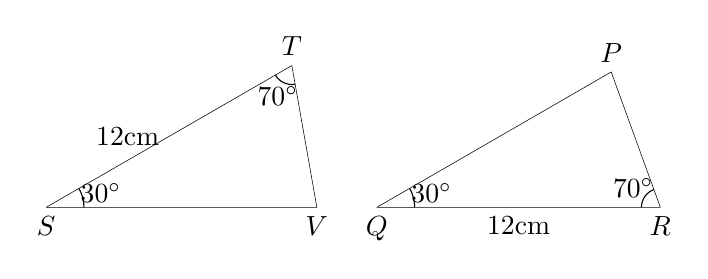
\begin{tikzpicture}[>=stealth,scale=0.6]
  \tkzSetUpPoint[fill=black]
  % \useasboundingbox(-1,-0.75)rectangle(3.7,1.4);
  \begin{scope}
  \tkzDefPoints{0/0/S, 5.2/3/T, 5.73/0/V}
  \tkzLabelPoints[below](S,V)
  \tkzLabelPoints[above](T)
  \tkzLabelSegment[left](S,T){12cm}
  \tkzMarkAngles[size=.8, mark=none](V,S,T)
  \tkzMarkAngles[size=.4, mark=none](S,T,V)
  \tkzLabelAngle[pos=1.2](V,S,T){$30^{\circ}$}
  \tkzLabelAngle[pos=.7](S,T,V){$70^{\circ}$}
  \tkzDrawPolygon(S,T,V)
  \end{scope}
  \begin{scope}[xshift=7cm]
    \tkzDefPoints{0/0/Q, 4.96/2.865/P, 6/0/R}
  \tkzLabelPoints[below](Q,R)
  \tkzLabelPoints[above](P)
  \tkzLabelSegment[below](Q,R){12cm}
  \tkzMarkAngles[size=.8, mark=none](R,Q,P)
  \tkzMarkAngles[size=.4, mark=none](P,R,Q)
  \tkzLabelAngle[pos=1.2](R,Q,P){$30^{\circ}$}
  \tkzLabelAngle[pos=.7](P,R,Q){$70^{\circ}$}
  \tkzDrawPolygon(P,R,Q)
  \end{scope}
\end{tikzpicture}
\end{document}